\documentclass{article}\usepackage[]{graphicx}\usepackage[]{xcolor}
% maxwidth is the original width if it is less than linewidth
% otherwise use linewidth (to make sure the graphics do not exceed the margin)
\makeatletter
\def\maxwidth{ %
  \ifdim\Gin@nat@width>\linewidth
    \linewidth
  \else
    \Gin@nat@width
  \fi
}
\makeatother

\definecolor{fgcolor}{rgb}{0.345, 0.345, 0.345}
\newcommand{\hlnum}[1]{\textcolor[rgb]{0.686,0.059,0.569}{#1}}%
\newcommand{\hlstr}[1]{\textcolor[rgb]{0.192,0.494,0.8}{#1}}%
\newcommand{\hlcom}[1]{\textcolor[rgb]{0.678,0.584,0.686}{\textit{#1}}}%
\newcommand{\hlopt}[1]{\textcolor[rgb]{0,0,0}{#1}}%
\newcommand{\hlstd}[1]{\textcolor[rgb]{0.345,0.345,0.345}{#1}}%
\newcommand{\hlkwa}[1]{\textcolor[rgb]{0.161,0.373,0.58}{\textbf{#1}}}%
\newcommand{\hlkwb}[1]{\textcolor[rgb]{0.69,0.353,0.396}{#1}}%
\newcommand{\hlkwc}[1]{\textcolor[rgb]{0.333,0.667,0.333}{#1}}%
\newcommand{\hlkwd}[1]{\textcolor[rgb]{0.737,0.353,0.396}{\textbf{#1}}}%
\let\hlipl\hlkwb

\usepackage{framed}
\makeatletter
\newenvironment{kframe}{%
 \def\at@end@of@kframe{}%
 \ifinner\ifhmode%
  \def\at@end@of@kframe{\end{minipage}}%
  \begin{minipage}{\columnwidth}%
 \fi\fi%
 \def\FrameCommand##1{\hskip\@totalleftmargin \hskip-\fboxsep
 \colorbox{shadecolor}{##1}\hskip-\fboxsep
     % There is no \\@totalrightmargin, so:
     \hskip-\linewidth \hskip-\@totalleftmargin \hskip\columnwidth}%
 \MakeFramed {\advance\hsize-\width
   \@totalleftmargin\z@ \linewidth\hsize
   \@setminipage}}%
 {\par\unskip\endMakeFramed%
 \at@end@of@kframe}
\makeatother

\definecolor{shadecolor}{rgb}{.97, .97, .97}
\definecolor{messagecolor}{rgb}{0, 0, 0}
\definecolor{warningcolor}{rgb}{1, 0, 1}
\definecolor{errorcolor}{rgb}{1, 0, 0}
\newenvironment{knitrout}{}{} % an empty environment to be redefined in TeX

\usepackage{alltt}
\title{\textbf{R Homework Three}}
\author{\textbf{Katherine Wolf}\\ Introduction to Causal Inference (PH252D)\\ \today}
\date{}

% list of latex packages you'll need
\usepackage{float}  % for tables
\usepackage{mathtools}  % for mathematical symbols
\usepackage{bm}  % to bold mathematical symbols like betas
\usepackage{scrextend}  % to indent subsections
\usepackage{xltxtra}
\usepackage{fontspec}
\usepackage{xunicode}
\usepackage[skip=0.5\baselineskip]{caption}  % control caption printing space
\usepackage{longtable}
\usepackage{amsfonts}
\usepackage{bm}
\usepackage{caption}
\usepackage[shortlabels]{enumitem}
\usepackage{txfonts}
\usepackage{dejavu}
\usepackage{mathpazo}
\usepackage{lmodern}
\usepackage{dirtytalk}
\usepackage{amsmath}

% set fonts
\setmainfont{Garamond}
\setsansfont{Lucida Console}

% set the margins of the document
\usepackage[top=1in, bottom=1in, left=.5in, right=.5in]{geometry}

% remove automatic indenting
\setlength{\parindent}{0pt}



% end the preamble and begin the document
\IfFileExists{upquote.sty}{\usepackage{upquote}}{}
\begin{document}

\maketitle

\section{Background and Causal Roadmap.}

\section{Import and explore the data set \texttt{RAssign4.csv}.}

  \subsection{Import the data set and assign it to object \texttt{ObsData}.}
  
\begin{knitrout}
\definecolor{shadecolor}{rgb}{0.969, 0.969, 0.969}\color{fgcolor}\begin{kframe}
\begin{alltt}
\hlkwd{library}\hlstd{(tidyverse)}

\hlstd{ObsData} \hlkwb{<-} \hlkwd{read.csv}\hlstd{(}\hlstr{"RAssign4.csv"}\hlstd{)}
\end{alltt}
\end{kframe}
\end{knitrout}

  \subsection{Assign the number of riders to \texttt{n}.}
  
\begin{knitrout}
\definecolor{shadecolor}{rgb}{0.969, 0.969, 0.969}\color{fgcolor}\begin{kframe}
\begin{alltt}
\hlstd{n} \hlkwb{<-} \hlkwd{nrow}\hlstd{(ObsData)}

\hlstd{n}
\end{alltt}
\begin{verbatim}
## [1] 5000
\end{verbatim}
\end{kframe}
\end{knitrout}

  \subsection{Use the \texttt{summary} function to explore the data.}
  
\begin{knitrout}
\definecolor{shadecolor}{rgb}{0.969, 0.969, 0.969}\color{fgcolor}\begin{kframe}
\begin{alltt}
\hlkwd{summary}\hlstd{(ObsData)}
\end{alltt}
\begin{verbatim}
##        W1              W2               A               Y        
##  Min.   :1.000   Min.   :0.0000   Min.   :1.000   Min.   :31.49  
##  1st Qu.:1.000   1st Qu.:0.0000   1st Qu.:3.000   1st Qu.:36.85  
##  Median :2.000   Median :0.0000   Median :4.000   Median :37.83  
##  Mean   :2.023   Mean   :0.3486   Mean   :4.085   Mean   :37.92  
##  3rd Qu.:3.000   3rd Qu.:1.0000   3rd Qu.:5.000   3rd Qu.:39.32  
##  Max.   :3.000   Max.   :1.0000   Max.   :7.000   Max.   :42.45
\end{verbatim}
\begin{alltt}
\hlkwd{tail}\hlstd{(ObsData)}
\end{alltt}
\begin{verbatim}
##      W1 W2 A        Y
## 4995  1  0 4 36.85538
## 4996  3  0 5 40.82337
## 4997  3  0 5 40.82456
## 4998  2  1 3 36.29618
## 4999  3  0 3 38.70285
## 5000  2  1 3 36.28475
\end{verbatim}
\end{kframe}
\end{knitrout}

  \subsection{Are there certain covariate combinations with limited variability in the exposure (burpees completed)?}
  
\begin{knitrout}
\definecolor{shadecolor}{rgb}{0.969, 0.969, 0.969}\color{fgcolor}\begin{kframe}
\begin{alltt}
\hlkwd{table}\hlstd{(ObsData}\hlopt{$}\hlstd{W1, ObsData}\hlopt{$}\hlstd{W2, ObsData}\hlopt{$}\hlstd{A)}
\end{alltt}
\begin{verbatim}
## , ,  = 1
## 
##    
##       0   1
##   1   2   6
##   2   7  20
##   3  25  40
## 
## , ,  = 2
## 
##    
##       0   1
##   1  40  50
##   2  56  80
##   3 114 132
## 
## , ,  = 3
## 
##    
##       0   1
##   1 130 124
##   2 174 156
##   3 281 223
## 
## , ,  = 4
## 
##    
##       0   1
##   1 266 175
##   2 348 172
##   3 324 145
## 
## , ,  = 5
## 
##    
##       0   1
##   1 318 127
##   2 320 117
##   3 249  63
## 
## , ,  = 6
## 
##    
##       0   1
##   1 232  57
##   2 156  28
##   3  99  12
## 
## , ,  = 7
## 
##    
##       0   1
##   1  69  10
##   2  36   5
##   3  11   1
\end{verbatim}
\end{kframe}
\end{knitrout}
  
    \subsubsection{Use the table function to check the number of riders in each exposure-covariate category.}
    
    \subsubsection{Comment.}
    
    \textcolor{red}{do this post-coding}

\section{IPTW for the statistical estimand estimand equal to the ATE under $\mathcal{M}^{\mathcal{F}^*}$}

  \subsection{We need to estimate the treatment mechanism $\mathbb{P}_0(A|W) = g_0(A|W)$, which is the conditional probability of completing $A$ burpees, given the rider's characteristics.} 

Implement the following code to estimate the treatment mechanism with multinomial logistic regression. You will need the \texttt{nnet} package:

\begin{knitrout}
\definecolor{shadecolor}{rgb}{0.969, 0.969, 0.969}\color{fgcolor}\begin{kframe}
\begin{alltt}
\hlkwd{library}\hlstd{(}\hlstr{"nnet"}\hlstd{)}
\end{alltt}


{\ttfamily\noindent\color{warningcolor}{\#\# Warning: package 'nnet' was built under R version 3.6.3}}\begin{alltt}
\hlstd{gAW.reg} \hlkwb{<-} \hlkwd{multinom}\hlstd{(A} \hlopt{~} \hlstd{W1} \hlopt{+} \hlstd{W2,}
                    \hlkwc{data} \hlstd{= ObsData)}
\end{alltt}
\begin{verbatim}
## # weights:  28 (18 variable)
## initial  value 9729.550745 
## iter  10 value 8205.693797
## iter  20 value 8032.285228
## final  value 8018.904637 
## converged
\end{verbatim}
\end{kframe}
\end{knitrout}
  
  \subsection{Predict each rider's probability of his/her observed exposure (burpees completed), given his/her covariates $\hat{g}(A_i|W_i)$:}
  
    \subsubsection{Use the \texttt{predict} function to obtain the predicted probability of each exposure level, given the rider's covariates. Be sure to specify \texttt{type = "probs"}.}
    
\begin{knitrout}
\definecolor{shadecolor}{rgb}{0.969, 0.969, 0.969}\color{fgcolor}\begin{kframe}
\begin{alltt}
\hlstd{gAW.pred} \hlkwb{<-} \hlkwd{predict}\hlstd{(gAW.reg,} \hlkwc{type}\hlstd{=}\hlstr{"probs"}\hlstd{)}
\end{alltt}
\end{kframe}
\end{knitrout}

    \subsubsection{Create an empty vector \texttt{gAW} of length \textit{n} for the predicted probabilities.}
    
\begin{knitrout}
\definecolor{shadecolor}{rgb}{0.969, 0.969, 0.969}\color{fgcolor}\begin{kframe}
\begin{alltt}
\hlstd{gAW} \hlkwb{<-} \hlkwd{rep}\hlstd{(}\hlnum{NA}\hlstd{, n)}
\end{alltt}
\end{kframe}
\end{knitrout}
    
    \subsubsection{Among riders with exposure level $A = 1$, assign the appropriate predicted probability:}
    
\begin{knitrout}
\definecolor{shadecolor}{rgb}{0.969, 0.969, 0.969}\color{fgcolor}\begin{kframe}
\begin{alltt}
\hlstd{gAW[ObsData}\hlopt{$}\hlstd{A}\hlopt{==}\hlnum{1}\hlstd{]} \hlkwb{<-} \hlstd{gAW.pred[ObsData}\hlopt{$}\hlstd{A}\hlopt{==}\hlnum{1}\hlstd{,} \hlstr{"1"}\hlstd{]}
\end{alltt}
\end{kframe}
\end{knitrout}
  
    \subsubsection{Implement the analogous code for exposure levels $A = 2, \ldots, A = 7$:}
    
\begin{knitrout}
\definecolor{shadecolor}{rgb}{0.969, 0.969, 0.969}\color{fgcolor}\begin{kframe}
\begin{alltt}
\hlstd{gAW[ObsData}\hlopt{$}\hlstd{A}\hlopt{==}\hlnum{2}\hlstd{]} \hlkwb{<-} \hlstd{gAW.pred[ObsData}\hlopt{$}\hlstd{A}\hlopt{==}\hlnum{2}\hlstd{,} \hlstr{"2"}\hlstd{]}

\hlstd{gAW[ObsData}\hlopt{$}\hlstd{A}\hlopt{==}\hlnum{3}\hlstd{]} \hlkwb{<-} \hlstd{gAW.pred[ObsData}\hlopt{$}\hlstd{A}\hlopt{==}\hlnum{3}\hlstd{,} \hlstr{"3"}\hlstd{]}

\hlstd{gAW[ObsData}\hlopt{$}\hlstd{A}\hlopt{==}\hlnum{4}\hlstd{]} \hlkwb{<-} \hlstd{gAW.pred[ObsData}\hlopt{$}\hlstd{A}\hlopt{==}\hlnum{4}\hlstd{,} \hlstr{"4"}\hlstd{]}

\hlstd{gAW[ObsData}\hlopt{$}\hlstd{A}\hlopt{==}\hlnum{5}\hlstd{]} \hlkwb{<-} \hlstd{gAW.pred[ObsData}\hlopt{$}\hlstd{A}\hlopt{==}\hlnum{5}\hlstd{,} \hlstr{"5"}\hlstd{]}

\hlstd{gAW[ObsData}\hlopt{$}\hlstd{A}\hlopt{==}\hlnum{6}\hlstd{]} \hlkwb{<-} \hlstd{gAW.pred[ObsData}\hlopt{$}\hlstd{A}\hlopt{==}\hlnum{6}\hlstd{,} \hlstr{"6"}\hlstd{]}

\hlstd{gAW[ObsData}\hlopt{$}\hlstd{A}\hlopt{==}\hlnum{7}\hlstd{]} \hlkwb{<-} \hlstd{gAW.pred[ObsData}\hlopt{$}\hlstd{A}\hlopt{==}\hlnum{7}\hlstd{,} \hlstr{"7"}\hlstd{]}
\end{alltt}
\end{kframe}
\end{knitrout}
    
    \subsubsection{Use the \texttt{summary} function to examine the distribution of predicted probabilities. Any cause for concern?}
    
\begin{knitrout}
\definecolor{shadecolor}{rgb}{0.969, 0.969, 0.969}\color{fgcolor}\begin{kframe}
\begin{alltt}
\hlkwd{summary}\hlstd{(gAW)}
\end{alltt}
\begin{verbatim}
##     Min.  1st Qu.   Median     Mean  3rd Qu.     Max. 
## 0.002224 0.175956 0.251250 0.228126 0.299407 0.341685
\end{verbatim}
\end{kframe}
\end{knitrout}

\textcolor{red}{talk about cause for concern after programming}
    
  \subsection{Create the vector \texttt{wt} as the inverse of the predicted probabilities. Use the \texttt{summary} function to examine the distribution of weights. Comment on the distribution of weights.}
  
\begin{knitrout}
\definecolor{shadecolor}{rgb}{0.969, 0.969, 0.969}\color{fgcolor}\begin{kframe}
\begin{alltt}
\hlstd{wt} \hlkwb{<-} \hlnum{1}\hlopt{/}\hlstd{gAW}
\hlkwd{summary}\hlstd{(wt)}
\end{alltt}
\begin{verbatim}
##    Min. 1st Qu.  Median    Mean 3rd Qu.    Max. 
##   2.927   3.340   3.980   6.934   5.683 449.690
\end{verbatim}
\end{kframe}
\end{knitrout}
  
\textcolor{red}{comment after programming}

  \subsection{Evaluate the IPTW estimand:}
  
\begin{align*}
\hat{\Psi}_{IPTW}(\mathbb{P}_n)=\frac{1}{n}\sum_{i=1}^{n}\frac{\mathbb{I}(A_i=7)}{\hat{g}(A_i|W_i)}Y_i - \frac{1}{n}\sum_{i=1}^{n}\frac{\mathbb{I}(A_i=1)}{\hat{g}(A_i|W_i)}Y_i
\end{align*}

The first quantity is the weighted mean outcome, where riders completing $A_i = 7$ burpees receive weight $\frac{1}{\hat{g}(A_i = 7 | W_i)}$ and riders completing $A_i \neq 7$ burpees receive weight 0. The second quantity is the weighted mean outcome, where riders completing $A_i = 1$ burpees receive weight $\frac{1}{\hat{g}(A_i = 1 | W_i)}$ and riders completing $A_i \neq 1$ burpees receive weight 0.

\begin{knitrout}
\definecolor{shadecolor}{rgb}{0.969, 0.969, 0.969}\color{fgcolor}\begin{kframe}
\begin{alltt}
\hlstd{iptw.estimand} \hlkwb{<-} \hlkwd{mean}\hlstd{(wt}\hlopt{*}\hlkwd{as.numeric}\hlstd{(ObsData}\hlopt{$}\hlstd{A}\hlopt{==}\hlnum{7}\hlstd{)}\hlopt{*}\hlstd{ObsData}\hlopt{$}\hlstd{Y)} \hlopt{-}
  \hlkwd{mean}\hlstd{(wt}\hlopt{*}\hlkwd{as.numeric}\hlstd{(ObsData}\hlopt{$}\hlstd{A}\hlopt{==}\hlnum{1}\hlstd{)}\hlopt{*}\hlstd{ObsData}\hlopt{$}\hlstd{Y)}

\hlstd{iptw.estimand}
\end{alltt}
\begin{verbatim}
## [1] 7.531834
\end{verbatim}
\end{kframe}
\end{knitrout}

  \subsection{Implement the stabilized IPTW estimator (a.k.a. the modified Horvitz-Thompson estimator):}
  
\begin{align*}
\hat{\Psi}_{st.IPTW}=
  \frac{\frac{1}{n}\sum_{i=1}^{n}\frac{\mathbb{I}(A_i=7)}{\hat{g}(A_i|W_i)}Y_i}{\frac{1}{n}\sum_{i=1}^{n}\frac{\mathbb{I}(A_i=7)}{\hat{g}(A_i|W_i)}} - 
  \frac{\frac{1}{n}\sum_{i=1}^{n}\frac{\mathbb{I}(A_i=1)}{\hat{g}(A_i|W_i)}Y_i}{\frac{1}{n}\sum_{i=1}^{n}\frac{\mathbb{I}(A_i=1)}{\hat{g}(A_i|W_i)}}
\end{align*}

\begin{knitrout}
\definecolor{shadecolor}{rgb}{0.969, 0.969, 0.969}\color{fgcolor}\begin{kframe}
\begin{alltt}
\hlstd{iptw.ht.estimand} \hlkwb{<-}
  \hlkwd{mean}\hlstd{(wt}\hlopt{*}\hlkwd{as.numeric}\hlstd{(ObsData}\hlopt{$}\hlstd{A}\hlopt{==}\hlnum{7}\hlstd{)}\hlopt{*}\hlstd{ObsData}\hlopt{$}\hlstd{Y)}\hlopt{/}
  \hlkwd{mean}\hlstd{(wt}\hlopt{*}\hlkwd{as.numeric}\hlstd{(ObsData}\hlopt{$}\hlstd{A}\hlopt{==}\hlnum{7}\hlstd{))} \hlopt{-}
  \hlkwd{mean}\hlstd{(wt}\hlopt{*}\hlkwd{as.numeric}\hlstd{(ObsData}\hlopt{$}\hlstd{A}\hlopt{==}\hlnum{1}\hlstd{)}\hlopt{*}\hlstd{ObsData}\hlopt{$}\hlstd{Y)}\hlopt{/}
  \hlkwd{mean}\hlstd{(wt}\hlopt{*}\hlkwd{as.numeric}\hlstd{(ObsData}\hlopt{$}\hlstd{A}\hlopt{==}\hlnum{1}\hlstd{))}
\end{alltt}
\end{kframe}
\end{knitrout}
  
  \subsection{Interpet the point estimates.}
  
\textcolor{red}{do this after programming}
  
\section{IPTW and Marginal Structural Models}

  \subsection{IPTW for the MSM parameter without stabilized weights}
  
    \subsubsection{Estimate the treatment mechanism $\mathbb{P}_0(A|W)=g_0(A|W)$, which is the conditional probability of completing $A$ burpees, given the rider's characteristics. Use multinomial logistic regression.
    \textit{Hint: We already did this! Skip to the next step.}}
    
    \subsubsection{Predict each rider's probability of her observed expsoure (burpees completed), given his/her covariates $\hat{g}(A_i|W_i)$. 
    \textit{Hint: We already did this! Skip to the next step.}}
    
    \subsubsection{Create the vector \texttt{wt} as the inverse of the predicted probabilities. 
    \textit{Hint: We already did this! Skip to the next step.}}
        
    \subsubsection{Estimate the parameters corresponding to the MSM by regressing the observed outcome $Y$ on the exposure $A$ according to $m(a|\beta)$. You must specify the \texttt{weights} and the \texttt{data}.}
    
\begin{knitrout}
\definecolor{shadecolor}{rgb}{0.969, 0.969, 0.969}\color{fgcolor}\begin{kframe}
\begin{alltt}
\hlstd{iptw.msm} \hlkwb{<-} \hlkwd{glm}\hlstd{(Y} \hlopt{~} \hlstd{A ,}
                \hlkwc{weights} \hlstd{= wt,}
                \hlkwc{data} \hlstd{= ObsData)}

\hlstd{iptw.msm}\hlopt{$}\hlstd{coef}
\end{alltt}
\begin{verbatim}
## (Intercept)           A 
##   33.084091    1.095612
\end{verbatim}
\begin{alltt}
\hlkwd{summary}\hlstd{(iptw.msm)}
\end{alltt}
\begin{verbatim}
## 
## Call:
## glm(formula = Y ~ A, data = ObsData, weights = wt)
## 
## Deviance Residuals: 
##     Min       1Q   Median       3Q      Max  
## -49.508   -1.338    1.428    2.470   15.694  
## 
## Coefficients:
##             Estimate Std. Error t value Pr(>|t|)    
## (Intercept) 33.08409    0.04657   710.4   <2e-16 ***
## A            1.09561    0.01043   105.1   <2e-16 ***
## ---
## Signif. codes:  0 '***' 0.001 '**' 0.01 '*' 0.05 '.' 0.1 ' ' 1
## 
## (Dispersion parameter for gaussian family taken to be 14.87555)
## 
##     Null deviance: 238519  on 4999  degrees of freedom
## Residual deviance:  74348  on 4998  degrees of freedom
## AIC: 19673
## 
## Number of Fisher Scoring iterations: 2
\end{verbatim}
\end{kframe}
\end{knitrout}
            
    \subsubsection{Interpret the results.}

\textcolor{red}{do after programming QUESTION: INCLUDE COVARIATES?}
    
  \subsection{IPTW for a MSM parameter with stabilized weights}
  
  \subsection{Implement IPTW for a MSM parameter with stabilized weights}
  
    \subsubsection{Estimate the treatment mechanism $g_0(A|W) = \mathbb{P}_0(A|W)$. 
    \textit{Hint: We already did this! Skip to the next step.}}
    
    \subsubsection{Predict the probability of the observed exposure for each rider \texttt{gAW}. 
    \textit{Hint: We already did this! Skip to the next step.}}
    
    \subsubsection{Create the stabilized weights \texttt{wt.MSM}:}
    
\begin{align*}
\frac{\hat{g}^*(A)}{\hat{g}(A|W)}, \; where \; \hat{g}^*(A) = \frac{1}{n}\sum_{i=1}^{n}\mathbb{I}(A_i=a)
\end{align*}

    \begin{enumerate}
      \item Create empty vector \texttt{gA} of length $n$ for the numerator of the weights.
      
\begin{knitrout}
\definecolor{shadecolor}{rgb}{0.969, 0.969, 0.969}\color{fgcolor}\begin{kframe}
\begin{alltt}
\hlstd{gA} \hlkwb{<-} \hlkwd{rep}\hlstd{(}\hlnum{NA}\hlstd{, n)}
\end{alltt}
\end{kframe}
\end{knitrout}
      
      \item Index the vector \texttt{gA} by exposure status and assign the appropriate estimated probability. \textit{Hint:} For riders completing $A=1$ burpee, the numerator $g^*(A)$ is the observed proportion with $A=1$.
      
\begin{knitrout}
\definecolor{shadecolor}{rgb}{0.969, 0.969, 0.969}\color{fgcolor}\begin{kframe}
\begin{alltt}
\hlstd{gA[ObsData}\hlopt{$}\hlstd{A}\hlopt{==}\hlnum{1}\hlstd{]} \hlkwb{<-} \hlkwd{mean}\hlstd{(ObsData}\hlopt{$}\hlstd{A}\hlopt{==}\hlnum{1}\hlstd{)}

\hlstd{gA[ObsData}\hlopt{$}\hlstd{A}\hlopt{==}\hlnum{2}\hlstd{]} \hlkwb{<-} \hlkwd{mean}\hlstd{(ObsData}\hlopt{$}\hlstd{A}\hlopt{==}\hlnum{2}\hlstd{)}

\hlstd{gA[ObsData}\hlopt{$}\hlstd{A}\hlopt{==}\hlnum{3}\hlstd{]} \hlkwb{<-} \hlkwd{mean}\hlstd{(ObsData}\hlopt{$}\hlstd{A}\hlopt{==}\hlnum{3}\hlstd{)}

\hlstd{gA[ObsData}\hlopt{$}\hlstd{A}\hlopt{==}\hlnum{4}\hlstd{]} \hlkwb{<-} \hlkwd{mean}\hlstd{(ObsData}\hlopt{$}\hlstd{A}\hlopt{==}\hlnum{4}\hlstd{)}

\hlstd{gA[ObsData}\hlopt{$}\hlstd{A}\hlopt{==}\hlnum{5}\hlstd{]} \hlkwb{<-} \hlkwd{mean}\hlstd{(ObsData}\hlopt{$}\hlstd{A}\hlopt{==}\hlnum{5}\hlstd{)}

\hlstd{gA[ObsData}\hlopt{$}\hlstd{A}\hlopt{==}\hlnum{6}\hlstd{]} \hlkwb{<-} \hlkwd{mean}\hlstd{(ObsData}\hlopt{$}\hlstd{A}\hlopt{==}\hlnum{6}\hlstd{)}

\hlstd{gA[ObsData}\hlopt{$}\hlstd{A}\hlopt{==}\hlnum{7}\hlstd{]} \hlkwb{<-} \hlkwd{mean}\hlstd{(ObsData}\hlopt{$}\hlstd{A}\hlopt{==}\hlnum{7}\hlstd{)}
\end{alltt}
\end{kframe}
\end{knitrout}
      
      \item Create the stabilized weights:
      
\begin{knitrout}
\definecolor{shadecolor}{rgb}{0.969, 0.969, 0.969}\color{fgcolor}\begin{kframe}
\begin{alltt}
\hlstd{wt.MSM} \hlkwb{<-} \hlstd{gA}\hlopt{/}\hlstd{gAW}
\end{alltt}
\end{kframe}
\end{knitrout}
    
      \item Comment on the distribution of the stabilized weights.
      
\textcolor{red}{do this post-programming}
    
    \end{enumerate}
    
  \subsubsection{Estimate the parameters corresponding to the MSM by regressing the observed outcome $Y$ on the exposure $A$. You must specify the \texttt{weights} and the \texttt{data}.}
  
\begin{knitrout}
\definecolor{shadecolor}{rgb}{0.969, 0.969, 0.969}\color{fgcolor}\begin{kframe}
\begin{alltt}
\hlstd{iptw.msm.st} \hlkwb{<-} \hlkwd{glm}\hlstd{(Y} \hlopt{~} \hlstd{A ,}
                   \hlkwc{weights} \hlstd{= wt.MSM,}
                   \hlkwc{data} \hlstd{= ObsData)}

\hlstd{iptw.msm.st}\hlopt{$}\hlstd{coef}
\end{alltt}
\begin{verbatim}
## (Intercept)           A 
##   33.671481    1.025057
\end{verbatim}
\begin{alltt}
\hlkwd{summary}\hlstd{(iptw.msm.st)}
\end{alltt}
\begin{verbatim}
## 
## Call:
## glm(formula = Y ~ A, data = ObsData, weights = wt.MSM)
## 
## Deviance Residuals: 
##     Min       1Q   Median       3Q      Max  
## -8.5159  -0.8660   0.3280   0.8466   2.4091  
## 
## Coefficients:
##             Estimate Std. Error t value Pr(>|t|)    
## (Intercept) 33.67148    0.06476  519.97   <2e-16 ***
## A            1.02506    0.01513   67.75   <2e-16 ***
## ---
## Signif. codes:  0 '***' 0.001 '**' 0.01 '*' 0.05 '.' 0.1 ' ' 1
## 
## (Dispersion parameter for gaussian family taken to be 1.945574)
## 
##     Null deviance: 18654  on 4999  degrees of freedom
## Residual deviance:  9724  on 4998  degrees of freedom
## AIC: 17901
## 
## Number of Fisher Scoring iterations: 2
\end{verbatim}
\end{kframe}
\end{knitrout}
  
  \subsubsection{Are the estimated coefficients the same? Briefly discuss.}
  
\textcolor{red}{do this post-programming}
  
\section{Improving the IPTW estimator and the G-computation formula}

  \subsection{Run the code given in \texttt{Rassign4\_modifiedIPTW.R} and report how the standard IPTW and modified Horvitz-Thompson estimators perform in terms of bias, variance, and MSE. Which estimator would you use in practice?}
  
\begin{knitrout}
\definecolor{shadecolor}{rgb}{0.969, 0.969, 0.969}\color{fgcolor}\begin{kframe}
\begin{alltt}
\hlkwd{source}\hlstd{(}\hlstr{"Rassign4_iptwModified.R"}\hlstd{)}
\end{alltt}
\begin{verbatim}
## [1] "The estimators have (estimated) bias:"
##          IPTW    Modifed HT   simple.mean        my.est      my.est.2 
##  4.990738e-01  2.180333e-04 -2.279129e-02 -7.738690e-06 -4.155064e-01 
## [1] "The estimators have (estimated) variance:"
##         IPTW   Modifed HT  simple.mean       my.est     my.est.2 
## 2.179920e+03 7.772966e-04 2.408178e-04 7.702404e-04 8.702269e-05 
## [1] "The estimators have (estimated) MSE:"
##         IPTW   Modifed HT  simple.mean       my.est     my.est.2 
## 2.180170e+03 7.773441e-04 7.602606e-04 7.702405e-04 1.727326e-01
\end{verbatim}
\end{kframe}
\end{knitrout}

The modified Horvitz-Thompson IPTW estimator has lower bias, variance, and mean squared error for this sample than the standard IPTW estimator, and I would likely use it in practice. That said, with a large enough sample, both estimators should be unbiased, but I would still likely use the Horvitz-Thompson estimator because it weights uncommon exposure-covariate combinations in the data (i.e., covariate combinations with small numbers of either exposed or unexposed observations) less heavily than standard IPTW estimator, which makes it less sensitive to theoretical and practical positivity violations, generally reduces its variance, and leads to better final sample performance than that of the standard IPTW estimator.

  \subsection{Look at the IPTW column in the \texttt{est} matrix. What do you notice about the IPTW estimates across these 2000 Monte Carlo draws?}
  
\begin{knitrout}
\definecolor{shadecolor}{rgb}{0.969, 0.969, 0.969}\color{fgcolor}\begin{kframe}
\begin{alltt}
\hlkwd{summary}\hlstd{(est[,}\hlstr{"IPTW"}\hlstd{])}
\end{alltt}
\begin{verbatim}
##    Min. 1st Qu.  Median    Mean 3rd Qu.    Max. 
##   863.0   968.1  1000.6  1001.1  1034.4  1145.7
\end{verbatim}
\begin{alltt}
\hlkwd{var}\hlstd{(est[,}\hlstr{"IPTW"}\hlstd{])}
\end{alltt}
\begin{verbatim}
## [1] 2179.92
\end{verbatim}
\begin{alltt}
\hlkwd{hist}\hlstd{(est[,}\hlstr{"IPTW"}\hlstd{])}
\end{alltt}
\end{kframe}
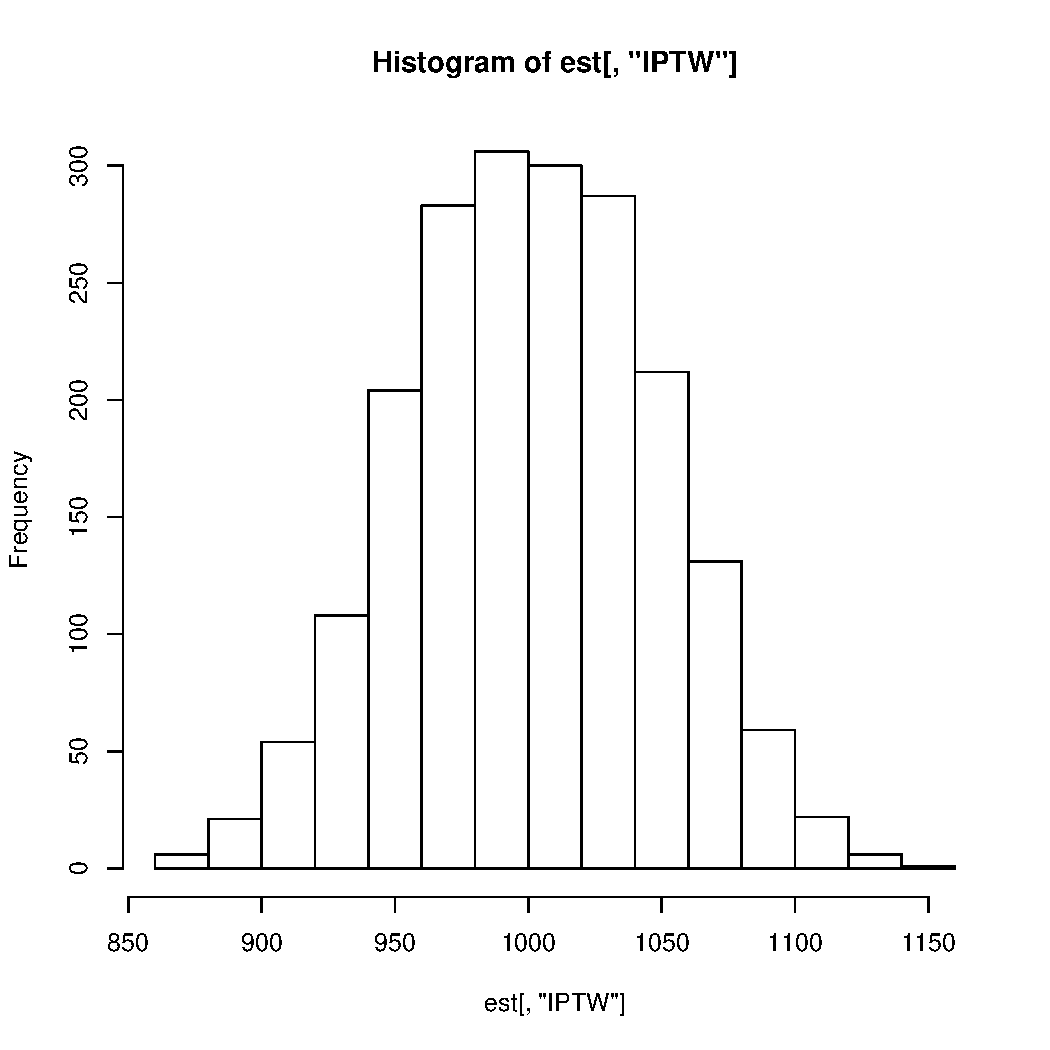
\includegraphics[width=\maxwidth]{figure/unnamed-chunk-21-1} 

\end{knitrout}
  
$Y$ can only take on one of two values, $Y = 1000$ or $Y = 1001$, but the IPTW estimates include $Y$ values ranging from 863.02 to 1145.69.
  
  \subsection{What is the variance of a random variable $X$ with $Pr(X = 0) = 1/2$ and $Pr(X = 1) = 1/2$?}
  
Such a random variable is a Bernoulli random variable with $p = Pr(X = 1) = 1/2$ and $q = Pr(X = 0) = 1/2$. Thus the mean of $X$ is $E[X]=\frac{1}{2}*1+\frac{1}{2}*0=\frac{1}{2}$, and the expected value of $X^2$ is $E[X^2] = \sum_{x\in range(X)}x^2(\mathbb{P}_x) = 1^2*\frac{1}{2}+0^2*\frac{1}{2} = \frac{1}{2}$. Since variance of a random variable is by defnition $Var[X]=E[(X-E[X])^2]=E[X^2]-(E[X])^2$, then the variance of our Bernoulli random variable friend $X$ is $Var[X] = E[X^2]-(E[X])^2 = \frac{1}{2} - (\frac{1}{2})^2 = \frac{1}{4}$.

  \subsection{What is the variance of a random variable $X2$ with $Pr(X2 = 0) = 1/2$ and $Pr(X2 = 1000) = 1/2$?}
  
The mean of such a variable would be $E[X2]=\sum_{x2\in range(X2)}x2(\mathbb{P}_x2) = \frac{1}{2}*0+\frac{1}{2}*1000 = 500$.

The expected value of the square of such a variable would be $E[X2^2]=\sum_{x2\in range(X2)}x2^2(\mathbb{P}_x2)=0^2*\frac{1}{2}+1000^2*\frac{1}{2} = \ensuremath{5\times 10^{5}}$.

Thus the variance of such a variable would be $Var[X2] = E[X2^2]-(E[X2])^2 = \ensuremath{5\times 10^{5}} - 500^2 = \ensuremath{2.5\times 10^{5}}$.
  
  \subsection{Can you think of how the above two calculations could be relevant to improving the IPTW estimator in this problem?}
  
If we find a way to reduce the range of the predicted Y values that the estimator averages to estimate $\psi(\mathbb{P}_0)$, the resulting estimator will be more efficient, i.e., its estimate will have a smaller variance, which could possibly reduce the ultimate mean squared error. 
  
  \subsection{\textit{Bonus:} Write down an estimator $\hat{\Psi}_{my.est}$ which applies the ideas of the previous three questions into an estimator. There's no need to give the best possible estimator, but you should give an estimator that outperforms the IPTW estimator by a significant margin (i.e. does as or almost as well as the modified Horvitz-Thompson estimator in terms of bias/variance/MSE).}
  
Below is the IPTW estimator stabilized by subracting the mean of the observed $Y$ values from each $Y_i$ and then adding that mean back at the end before calculating the overall mean.
  
\begin{align*}
\hat{\psi}_{katie}(\mathbb{P}_n)=\frac{1}{n}\sum_{i=1}^{n}[\frac{A_i(Y_i-\sum_{i=1}^{n}(Y_i))}{g_0(1|W_i)}+\sum_{i=1}^{n}(Y_i)]
\end{align*}
  
  \subsection{\textit{Bonus:} Code your estimator and replace the NA on the line \texttt{my.est = NA} with the estimator you defined in the previous question. Report the bias/variance/MSE of your estimator over the 2000 Monte Carlo draws.}

\begin{knitrout}
\definecolor{shadecolor}{rgb}{0.969, 0.969, 0.969}\color{fgcolor}\begin{kframe}
\begin{alltt}
\hlkwd{source}\hlstd{(}\hlstr{"Rassign4_iptwModified.R"}\hlstd{)}
\end{alltt}
\begin{verbatim}
## [1] "The estimators have (estimated) bias:"
##          IPTW    Modifed HT   simple.mean        my.est      my.est.2 
##  4.990738e-01  2.180333e-04 -2.279129e-02 -7.738690e-06 -4.155064e-01 
## [1] "The estimators have (estimated) variance:"
##         IPTW   Modifed HT  simple.mean       my.est     my.est.2 
## 2.179920e+03 7.772966e-04 2.408178e-04 7.702404e-04 8.702269e-05 
## [1] "The estimators have (estimated) MSE:"
##         IPTW   Modifed HT  simple.mean       my.est     my.est.2 
## 2.180170e+03 7.773441e-04 7.602606e-04 7.702405e-04 1.727326e-01
\end{verbatim}
\end{kframe}
\end{knitrout}

My estimator beats both the standard IPTW and modified modified Horvitz-Thompson estimator in bias, variance, and mean squared error! It fails, however, to beat taking a simple mean of the observed Y values in terms of mean square error.

\end{document}
